\subsubsection*{Grafici e traiettorie}

La traccia lasciata da un aeroplano trattiene nel tempo la memoria del recente passaggio.\newline
In generale, si definisce {\bfseries traiettoria} l'insieme dei punti dello spazio occupati da un oggetto durante il proprio movimento.\newline
La traiettoria, tuttavia, offre una rappresentazione parziale del movimento. Osservando il solco tracciato su una pista di terra da una bicicletta non è possibile comprendere se il ciclista stesse pedalando lentamente o a ritmo sostenuto. Per una descrizione completa, è necessario acquisire anche informazioni relative agli istanti nei quali l'oggetto in movimento ha occupato ciascuna posizione.
\newline

Una descrizione completa di un moto è una {\bf \slshape funzione dello spazio nel tempo}, nella quale ad ogni singolo istante è associata la posizione occupata dall'oggetto nello spazio.
\newline

Di solito la rappresentazione di un moto è un'attività complessa, perché lo spazio è un'entità tridimensionale e richiede quindi la definizione di una funzione a 3 valori.
Tuttavia, siccome ciascuna posizione può essere scomposta nelle proprie componenti unidimensionali, è utile occuparsi, all'inizio, del cosidetto {\bf \slshape moto lineare}, nel quale la traiettoria del corpo è un {\bf \slshape sottoinsieme} della retta.
\newline

Per rappresentare il moto lineare, è particolarmente efficace riportare la traiettoria sull'asse verticale del piano cartesiano e il tempo su quello orizzontale. I punti di questo piano (che non sono nè punti dello spazio, nè istanti del tempo, proprio perché composti da una coordinata spaziale e da una coordinata temporale) vengono chiamati {\bf eventi}.

Pertanto, l'osservazione di un moto consiste nel rilievo di un certo numero finito di eventi discreti \footnote{spesso, nel linguaggio scientifico, il termine {\slshape discreto} è utilizzato come sinonimo di {\slshape separato} o {\slshape distinto}.}.
Se rappresentiamo gli eventi che descrivono un moto reale su un grafico spazio-tempo, possiamo fare delle osservazioni globali, che permettono di descrivere le caratteristiche del moto nel suo insieme.\newline

Il primo elemento importante da riconoscere è la distanza temporale che separa, a coppie, gli eventi nel tempo, che viene chiamata è chiamata intervallo di tempo ed è indicata spesso dal simbolo $\Delta t$:
\begin{center}
\begin{math}
\Delta t = t_{finale}-t_{iniziale}
\end{math}
\end{center}
Allo stesso modo, è importante verificare se il corpo, durante l'osservazione, ha modificato la propria posizione. Si può definire quindi lo spostamento $\Delta s$ come:
\begin{center}
\begin{math}
\Delta s = s_{finale} - s_{iniziale}
\end{math}
\end{center}
Per ogni coppia di eventi del grafico spazio tempo, si definisce {\bf velocità media} il rapporto tra lo spazio percorso e il tempo impiegato:
\begin{center}
\begin{equation}
v_{media}=\frac {\Delta s}{\Delta t}=\frac {s_{finale} -s_{iniziale}}{t_{finale}-t_{iniziale}}
\end{equation}
\end{center}
La velocità media è una proprietà associata esclusivmente due eventi - evento iniziale ed evento finale - che intervengono nella definizione. Se una automobile percorre dieci chilometri in dieci minuti, non possiamo sostenere che abbia transitato in tutti i punti del proprio percorso alla velocità di $60 \frac {km}{h}$, senza neppure fermarsi ai semafori. Tuttavia, l'osservazione di un campione abbastanza nutrito di eventi, sufficientemente ravvicinati nel tempo, ci induce qualche volta ad avanzare delle ipotesi relative ad eventi per quali non è stata operata una misura reale.
\newline

Supponiamo di rilevare alcuni passaggi di un podista sulla linea di arrivo di una pista di atletica, durante una gara su diecimila metri, e di riportarli su una tabella come la seguente:
\begin{center}
\begin{tabular}{| c | c |}
\hline
giri di pista & intervallo di tempo (s) \\
\hline
7° &  0 \\
\hline
9° & 144 \\
\hline
12° & 360 \\
\hline
16° & 648 \\
\hline
18° & 792 \\
\hline
23° & 1142 \\
\hline
\end{tabular}
\end{center}

In questo esempio, la rilevazione è cominciata al settimo giro di pista, quando il podista aveva già percorso 2800 metri (sette giri, appunto). I successivi rilievi riportano il tempo misurato a partire dal settimo giro. Ecco come può essere rappresentato il moto con geogebra:
\begin{figure}[H]
 \centering
 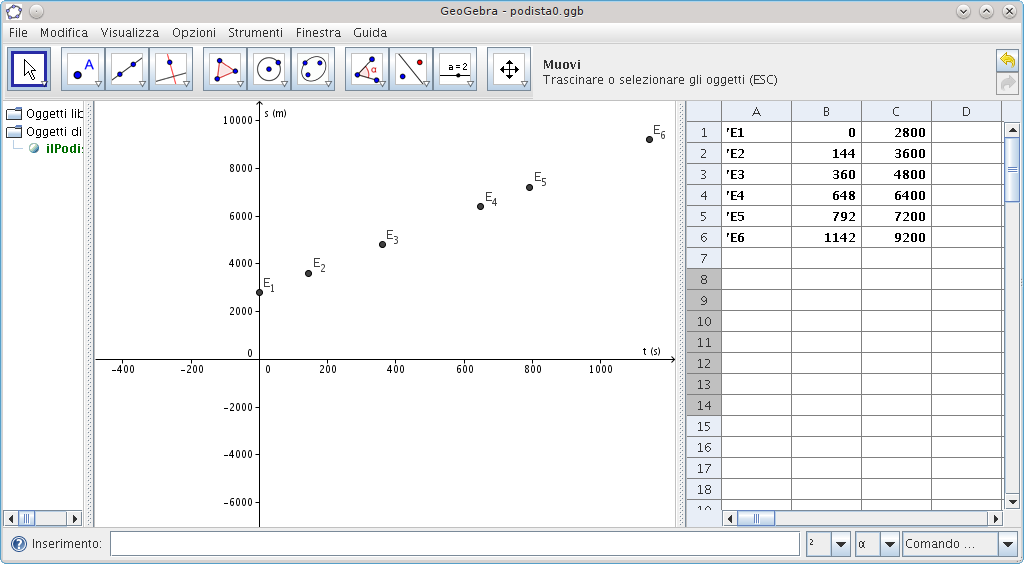
\includegraphics[width=.7\textwidth]{../immagini/podista.png}
 % podista.png
 \label{fig:il grafico spazio tempo di un podista}
\end{figure}

A prima vista, i punti appaiono ben allineati. Valutiamo, per alcune coppie di punti, i valori degli incrementi e delle velocità relative.
\begin{figure}[H]
 \centering
 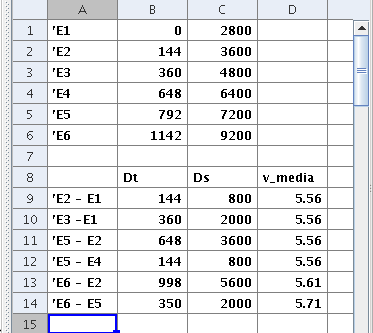
\includegraphics[width=.7\textwidth]{../immagini/podista1.png}
 % podista.png
 \label{fig:il grafico spazio tempo di un podista}
\end{figure}

In questo esempio, sono stati scelti soltanto alcuni dei possibili accoppiamenti tra i sei punti dell'esempio. Possiamo osservare, tuttavia, che la terza colonna, relativa alle velocità medie, contiene valori identici per tutti gli accoppiamenti, tranne che per le coppie di eventi in cui compare l'evento $E_6$, che contiene valori leggermente più alti.\newline
Questi calcoli ci portano a dedurre che il podista possa aver marciato fino al diciottesimo giro ad una velocità costante, e abbia incrementato leggermente il ritmo nei seguenti cinque giri.\newline
A questo punto, potremmo verificare con più attenzione l'allineamento dei punti del grafico, e osserveremmo che l'ultimo si discosta leggermente dalla linea dei precedenti.
\newline

Viene spontaneo, a questo punto, constatare l'analogia tra il concetto di velocità e il concetti di coefficiente angolare usato per descrivere la direzione delle rette nello spazio. In un grafico spazio-tempo, infatti, la velocità media tra due eventi è rappresentata dall'inclinazione del segmento che li unisce.
\newline

Osserviamo ancora i primi cinque punti del grafico. Come già detto, siccome sono tutti perfettamente allineati, ogni coppia di eventi definisce una velocità media uguale a tutte le altre, pari a $5,56 \frac ms$. Il fatto suggerisce l'ipotesi che il podista abbia rispettato la stessa condizione per tutti gli istanti compresi dal settimo al sedicesimo giro. Sulla base di questa assunzione, possiamo realizzare un modello del moto, tracciando una retta che unisca i cinque punti. Per farlo, basta utilizzare l'equazione $(4)$ del capitolo precedente, scrivendo:
\begin{center}
\begin{equation}
\label{eq:Equazione oraria del moto lineare uniforme}
s = s_0 + v (t -t_0)
\end{equation}
\end{center}
Questa equazione si chiama {\bf Equazione oraria del moto lineare uniforme}.\newline
che nel nostro caso diventa:
\begin{center}
\begin{math}
s = 2800 + 5.56 t
\end{math}
\end{center}
Confrontiamo graficamente i dati sperimentali con il modello teorico:
\begin{figure}[H]
 \centering
 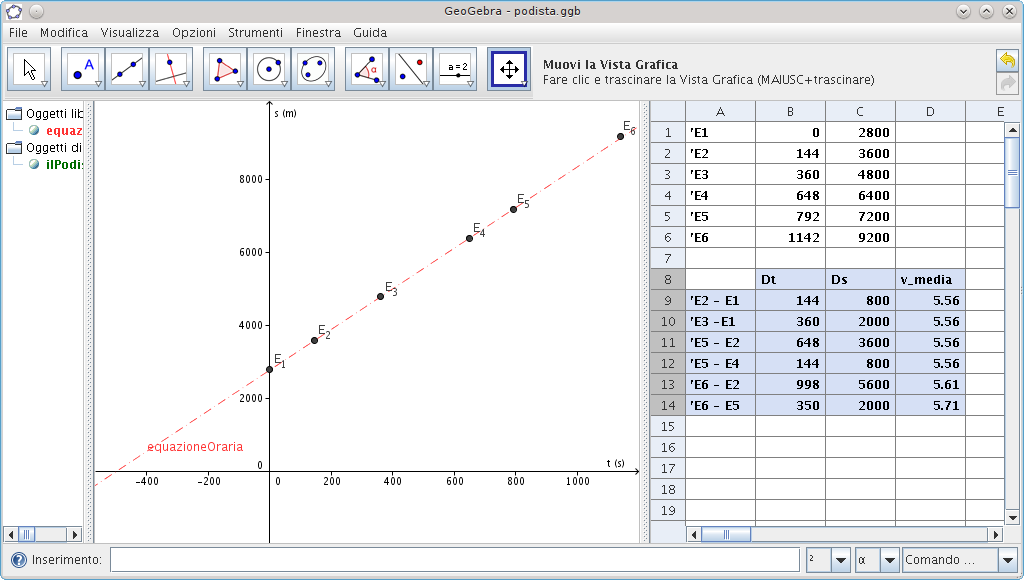
\includegraphics[width=.7\textwidth]{../immagini/podista2.png}
 % podista.png
 \label{fig:confronto dei dati con il modello}
\end{figure}


L'equazione data, ci permette di effettuare operazioni di interpolazione e di estrapolazione. Se ad esempio, ci chiediamo dopo quanto tempo il nostro modello prevede il passaggio del podista al decimo giro, possiamo semplicemente sostituire la posizione 4000 all'equazione oraria e ricavare il tempo $t$ come incognita:
\begin{center}
\begin{math}
t = \frac {s -s_0} {v} = \frac {4000 - 2800} {5.56} = 216 s
\end{math}
\end{center}
Siccome l'evento $(216;4000)$ è compreso all'interno dei cinque punti rilevati, parleremmo in questo caso di interpolazione.\newline
Potremmo invece effettuare delle estrapolazioni se desiderassimo valutare, sulla base del nostro modello, il tempo in cui avremmo atteso il passaggio del podista al ventitreesimo giro o il tempo di partenza della gara:
\begin{center}
\begin{math}
t = \frac {s -s_0} {v} = \frac {9200 - 2800} {5.56} = 1152 s
\end{math}
\end{center}
Il tempo atteso al ventitreesimo giro sarebbe stato 1152 s. Il podista, quindi, è transitato con un anticipo di 10 secondi, rispetto al modello teorico.
\begin{center}
\begin{math}
t = \frac {s -s_0} {v} = \frac {0 - 2800} {5.56} = - 504 s
\end{math}
\end{center}
Il tempo stimato di avvio della gara precede di 504 secondi il passaggio al settimo giro.
\newline

Il modello  che abbiamo utilizzato in questo esempio è un modello di {\bf moto a velocità constante}.
La velocità di uno spostamento è costante se, preso comunque un intervallo di tempo, la velocità media relativa agli estremi di quell'intervallo è sempre la stessa.\newline
Il concetto di velocità costante sottende quello di {\bf velocità istantanea}. Se un moto avviene a velocità constante, infatti, possiamo cosiderare la velocità come una proprietà di ciascun instante del moto, preso singolarmente. In seguito, renderemo più generale questo concetto per applicarlo a moti a velocità variabile.
